\documentclass[1p]{elsarticle_modified}
%\bibliographystyle{elsarticle-num}

%\usepackage[colorlinks]{hyperref}
%\usepackage{abbrmath_seonhwa} %\Abb, \Ascr, \Acal ,\Abf, \Afrak
\usepackage{amsfonts}
\usepackage{amssymb}
\usepackage{amsmath}
\usepackage{amsthm}
\usepackage{scalefnt}
\usepackage{amsbsy}
\usepackage{kotex}
\usepackage{caption}
\usepackage{subfig}
\usepackage{color}
\usepackage{graphicx}
\usepackage{xcolor} %% white, black, red, green, blue, cyan, magenta, yellow
\usepackage{float}
\usepackage{setspace}
\usepackage{hyperref}

\usepackage{tikz}
\usetikzlibrary{arrows}

\usepackage{multirow}
\usepackage{array} % fixed length table
\usepackage{hhline}

%%%%%%%%%%%%%%%%%%%%%
\makeatletter
\renewcommand*\env@matrix[1][\arraystretch]{%
	\edef\arraystretch{#1}%
	\hskip -\arraycolsep
	\let\@ifnextchar\new@ifnextchar
	\array{*\c@MaxMatrixCols c}}
\makeatother %https://tex.stackexchange.com/questions/14071/how-can-i-increase-the-line-spacing-in-a-matrix
%%%%%%%%%%%%%%%

\usepackage[normalem]{ulem}

\newcommand{\msout}[1]{\ifmmode\text{\sout{\ensuremath{#1}}}\else\sout{#1}\fi}
%SOURCE: \msout is \stkout macro in https://tex.stackexchange.com/questions/20609/strikeout-in-math-mode

\newcommand{\cancel}[1]{
	\ifmmode
	{\color{red}\msout{#1}}
	\else
	{\color{red}\sout{#1}}
	\fi
}

\newcommand{\add}[1]{
	{\color{blue}\uwave{#1}}
}

\newcommand{\replace}[2]{
	\ifmmode
	{\color{red}\msout{#1}}{\color{blue}\uwave{#2}}
	\else
	{\color{red}\sout{#1}}{\color{blue}\uwave{#2}}
	\fi
}

\newcommand{\Sol}{\mathcal{S}} %segment
\newcommand{\D}{D} %diagram
\newcommand{\A}{\mathcal{A}} %arc


%%%%%%%%%%%%%%%%%%%%%%%%%%%%%5 test

\def\sl{\operatorname{\textup{SL}}(2,\Cbb)}
\def\psl{\operatorname{\textup{PSL}}(2,\Cbb)}
\def\quan{\mkern 1mu \triangleright \mkern 1mu}

\theoremstyle{definition}
\newtheorem{thm}{Theorem}[section]
\newtheorem{prop}[thm]{Proposition}
\newtheorem{lem}[thm]{Lemma}
\newtheorem{ques}[thm]{Question}
\newtheorem{cor}[thm]{Corollary}
\newtheorem{defn}[thm]{Definition}
\newtheorem{exam}[thm]{Example}
\newtheorem{rmk}[thm]{Remark}
\newtheorem{alg}[thm]{Algorithm}

\newcommand{\I}{\sqrt{-1}}
\begin{document}

%\begin{frontmatter}
%
%\title{Boundary parabolic representations of knots up to 8 crossings}
%
%%% Group authors per affiliation:
%\author{Yunhi Cho} 
%\address{Department of Mathematics, University of Seoul, Seoul, Korea}
%\ead{yhcho@uos.ac.kr}
%
%
%\author{Seonhwa Kim} %\fnref{s_kim}}
%\address{Center for Geometry and Physics, Institute for Basic Science, Pohang, 37673, Korea}
%\ead{ryeona17@ibs.re.kr}
%
%\author{Hyuk Kim}
%\address{Department of Mathematical Sciences, Seoul National University, Seoul 08826, Korea}
%\ead{hyukkim@snu.ac.kr}
%
%\author{Seokbeom Yoon}
%\address{Department of Mathematical Sciences, Seoul National University, Seoul, 08826,  Korea}
%\ead{sbyoon15@snu.ac.kr}
%
%\begin{abstract}
%We find all boundary parabolic representation of knots up to 8 crossings.
%
%\end{abstract}
%\begin{keyword}
%    \MSC[2010] 57M25 
%\end{keyword}
%
%\end{frontmatter}

%\linenumbers
%\tableofcontents
%
\newcommand\colored[1]{\textcolor{white}{\rule[-0.35ex]{0.8em}{1.4ex}}\kern-0.8em\color{red} #1}%
%\newcommand\colored[1]{\textcolor{white}{ #1}\kern-2.17ex	\textcolor{white}{ #1}\kern-1.81ex	\textcolor{white}{ #1}\kern-2.15ex\color{red}#1	}

{\Large $\underline{12a_{0398}~(K12a_{0398})}$}

\setlength{\tabcolsep}{10pt}
\renewcommand{\arraystretch}{1.6}
\vspace{1cm}\begin{tabular}{m{100pt}>{\centering\arraybackslash}m{274pt}}
\multirow{5}{120pt}{
	\centering
	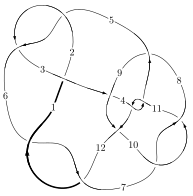
\includegraphics[width=112pt]{../../../GIT/diagram.site/Diagrams/png/1199_12a_0398.png}\\
\ \ \ A knot diagram\footnotemark}&
\allowdisplaybreaks
\textbf{Linearized knot diagam} \\
\cline{2-2}
 &
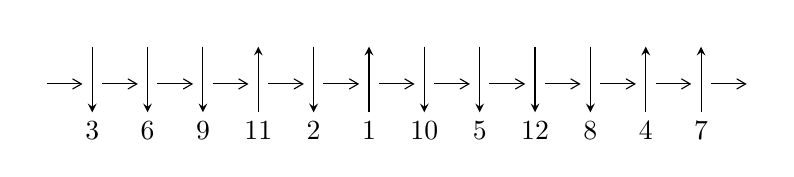
\begin{tikzpicture}[x=20pt, y=17pt]
	% nodes
	\node (C0) at (0, 0) {};
	\node (C1) at (1, 0) {};
	\node (C1U) at (1, +1) {};
	\node (C1D) at (1, -1) {3};

	\node (C2) at (2, 0) {};
	\node (C2U) at (2, +1) {};
	\node (C2D) at (2, -1) {6};

	\node (C3) at (3, 0) {};
	\node (C3U) at (3, +1) {};
	\node (C3D) at (3, -1) {9};

	\node (C4) at (4, 0) {};
	\node (C4U) at (4, +1) {};
	\node (C4D) at (4, -1) {11};

	\node (C5) at (5, 0) {};
	\node (C5U) at (5, +1) {};
	\node (C5D) at (5, -1) {2};

	\node (C6) at (6, 0) {};
	\node (C6U) at (6, +1) {};
	\node (C6D) at (6, -1) {1};

	\node (C7) at (7, 0) {};
	\node (C7U) at (7, +1) {};
	\node (C7D) at (7, -1) {10};

	\node (C8) at (8, 0) {};
	\node (C8U) at (8, +1) {};
	\node (C8D) at (8, -1) {5};

	\node (C9) at (9, 0) {};
	\node (C9U) at (9, +1) {};
	\node (C9D) at (9, -1) {12};

	\node (C10) at (10, 0) {};
	\node (C10U) at (10, +1) {};
	\node (C10D) at (10, -1) {8};

	\node (C11) at (11, 0) {};
	\node (C11U) at (11, +1) {};
	\node (C11D) at (11, -1) {4};

	\node (C12) at (12, 0) {};
	\node (C12U) at (12, +1) {};
	\node (C12D) at (12, -1) {7};
	\node (C13) at (13, 0) {};

	% arrows
	\draw[->,>={angle 60}]
	(C0) edge (C1) (C1) edge (C2) (C2) edge (C3) (C3) edge (C4) (C4) edge (C5) (C5) edge (C6) (C6) edge (C7) (C7) edge (C8) (C8) edge (C9) (C9) edge (C10) (C10) edge (C11) (C11) edge (C12) (C12) edge (C13) ;	\draw[->,>=stealth]
	(C1U) edge (C1D) (C2U) edge (C2D) (C3U) edge (C3D) (C4D) edge (C4U) (C5U) edge (C5D) (C6D) edge (C6U) (C7U) edge (C7D) (C8U) edge (C8D) (C9U) edge (C9D) (C10U) edge (C10D) (C11D) edge (C11U) (C12D) edge (C12U) ;
	\end{tikzpicture} \\
\hhline{~~} \\& 
\textbf{Solving Sequence} \\ \cline{2-2} 
 &
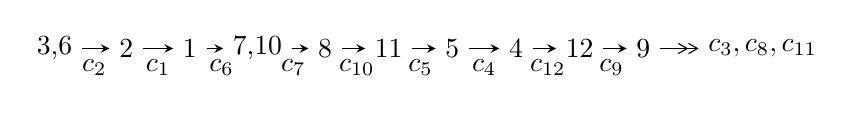
\begin{tikzpicture}[x=23pt, y=7pt]
	% node
	\node (A0) at (-1/8, 0) {3,6};
	\node (A1) at (1, 0) {2};
	\node (A2) at (2, 0) {1};
	\node (A3) at (49/16, 0) {7,10};
	\node (A4) at (33/8, 0) {8};
	\node (A5) at (41/8, 0) {11};
	\node (A6) at (49/8, 0) {5};
	\node (A7) at (57/8, 0) {4};
	\node (A8) at (65/8, 0) {12};
	\node (A9) at (73/8, 0) {9};
	\node (C1) at (1/2, -1) {$c_{2}$};
	\node (C2) at (3/2, -1) {$c_{1}$};
	\node (C3) at (5/2, -1) {$c_{6}$};
	\node (C4) at (29/8, -1) {$c_{7}$};
	\node (C5) at (37/8, -1) {$c_{10}$};
	\node (C6) at (45/8, -1) {$c_{5}$};
	\node (C7) at (53/8, -1) {$c_{4}$};
	\node (C8) at (61/8, -1) {$c_{12}$};
	\node (C9) at (69/8, -1) {$c_{9}$};
	\node (A10) at (11, 0) {$c_{3},c_{8},c_{11}$};

	% edge
	\draw[->,>=stealth]	
	(A0) edge (A1) (A1) edge (A2) (A2) edge (A3) (A3) edge (A4) (A4) edge (A5) (A5) edge (A6) (A6) edge (A7) (A7) edge (A8) (A8) edge (A9) ;
	\draw[->>,>={angle 60}]	
	(A9) edge (A10);
\end{tikzpicture} \\ 

\end{tabular} \\

\footnotetext{
The image of knot diagram is generated by the software ``\textbf{Draw programme}" developed by Andrew Bartholomew(\url{http://www.layer8.co.uk/maths/draw/index.htm\#Running-draw}), where we modified some parts for our purpose(\url{https://github.com/CATsTAILs/LinksPainter}).
}\phantom \\ \newline 
\centering \textbf{Ideals for irreducible components\footnotemark of $X_{\text{par}}$} 
 
\begin{align*}
I^u_{1}&=\langle 
-4.97226\times10^{50} u^{97}+4.65765\times10^{50} u^{96}+\cdots+9.94685\times10^{49} b+3.19075\times10^{50},\\
\phantom{I^u_{1}}&\phantom{= \langle  }7.33977\times10^{49} u^{97}-8.07721\times10^{49} u^{96}+\cdots+2.98406\times10^{50} a+7.44119\times10^{50},\;u^{98}-2 u^{97}+\cdots-5 u+1\rangle \\
I^u_{2}&=\langle 
5 u^5-3 u^4-7 u^3+8 u^2+17 b+11 u+1,\;4 u^5-16 u^4-26 u^3+20 u^2+17 a+19 u-6,\\
\phantom{I^u_{2}}&\phantom{= \langle  }u^6+u^5- u^4-2 u^3+u+1\rangle \\
\\
\end{align*}
\raggedright * 2 irreducible components of $\dim_{\mathbb{C}}=0$, with total 104 representations.\\
\footnotetext{All coefficients of polynomials are rational numbers. But the coefficients are sometimes approximated in decimal forms when there is not enough margin.}
\newpage
\renewcommand{\arraystretch}{1}
\centering \section*{I. $I^u_{1}= \langle -4.97\times10^{50} u^{97}+4.66\times10^{50} u^{96}+\cdots+9.95\times10^{49} b+3.19\times10^{50},\;7.34\times10^{49} u^{97}-8.08\times10^{49} u^{96}+\cdots+2.98\times10^{50} a+7.44\times10^{50},\;u^{98}-2 u^{97}+\cdots-5 u+1 \rangle$}
\flushleft \textbf{(i) Arc colorings}\\
\begin{tabular}{m{7pt} m{180pt} m{7pt} m{180pt} }
\flushright $a_{3}=$&$\begin{pmatrix}1\\0\end{pmatrix}$ \\
\flushright $a_{6}=$&$\begin{pmatrix}0\\u\end{pmatrix}$ \\
\flushright $a_{2}=$&$\begin{pmatrix}1\\- u^2\end{pmatrix}$ \\
\flushright $a_{1}=$&$\begin{pmatrix}- u^2+1\\- u^2\end{pmatrix}$ \\
\flushright $a_{7}=$&$\begin{pmatrix}u^5-2 u^3+u\\u^5- u^3+u\end{pmatrix}$ \\
\flushright $a_{10}=$&$\begin{pmatrix}-0.245966 u^{97}+0.270679 u^{96}+\cdots-0.544659 u-2.49365\\4.99882 u^{97}-4.68254 u^{96}+\cdots+17.2389 u-3.20780\end{pmatrix}$ \\
\flushright $a_{8}=$&$\begin{pmatrix}0.293712 u^{97}-0.601992 u^{96}+\cdots+4.46853 u-2.86203\\4.85358 u^{97}-4.20830 u^{96}+\cdots+16.6402 u-2.74961\end{pmatrix}$ \\
\flushright $a_{11}=$&$\begin{pmatrix}-0.979346 u^{97}+1.70885 u^{96}+\cdots-8.77351 u+0.791545\\0.216714 u^{97}-0.560914 u^{96}+\cdots+0.966260 u-0.417735\end{pmatrix}$ \\
\flushright $a_{5}=$&$\begin{pmatrix}u\\- u^3+u\end{pmatrix}$ \\
\flushright $a_{4}=$&$\begin{pmatrix}2.87151 u^{97}-2.46999 u^{96}+\cdots+7.08329 u-1.86426\\-0.626345 u^{97}+0.422548 u^{96}+\cdots-3.41997 u+1.08263\end{pmatrix}$ \\
\flushright $a_{12}=$&$\begin{pmatrix}- u^8+3 u^6-3 u^4+1\\- u^8+2 u^6-2 u^4\end{pmatrix}$ \\
\flushright $a_{9}=$&$\begin{pmatrix}-5.41930 u^{97}+6.52843 u^{96}+\cdots-21.8687 u+3.43085\\1.32970 u^{97}-1.22300 u^{96}+\cdots+6.06795 u-0.752344\end{pmatrix}$\\&\end{tabular}
\flushleft \textbf{(ii) Obstruction class $= -1$}\\~\\
\flushleft \textbf{(iii) Cusp Shapes $= 1.95346 u^{97}+1.64120 u^{96}+\cdots-1.69682 u-8.13481$}\\~\\
\newpage\renewcommand{\arraystretch}{1}
\flushleft \textbf{(iv) u-Polynomials at the component}\newline \\
\begin{tabular}{m{50pt}|m{274pt}}
Crossings & \hspace{64pt}u-Polynomials at each crossing \\
\hline $$\begin{aligned}c_{1}\end{aligned}$$&$\begin{aligned}
&u^{98}+54 u^{97}+\cdots+15 u+1
\end{aligned}$\\
\hline $$\begin{aligned}c_{2},c_{5}\end{aligned}$$&$\begin{aligned}
&u^{98}+2 u^{97}+\cdots+5 u+1
\end{aligned}$\\
\hline $$\begin{aligned}c_{3}\end{aligned}$$&$\begin{aligned}
&u^{98}- u^{97}+\cdots+56576 u-18496
\end{aligned}$\\
\hline $$\begin{aligned}c_{4},c_{11}\end{aligned}$$&$\begin{aligned}
&u^{98}-2 u^{97}+\cdots+u+1
\end{aligned}$\\
\hline $$\begin{aligned}c_{6},c_{12}\end{aligned}$$&$\begin{aligned}
&u^{98}+6 u^{97}+\cdots-585 u-117
\end{aligned}$\\
\hline $$\begin{aligned}c_{7},c_{10}\end{aligned}$$&$\begin{aligned}
&u^{98}-7 u^{97}+\cdots-1854 u-289
\end{aligned}$\\
\hline $$\begin{aligned}c_{8}\end{aligned}$$&$\begin{aligned}
&17(17 u^{98}+153 u^{97}+\cdots-1.14403\times10^{7} u-3023343)
\end{aligned}$\\
\hline $$\begin{aligned}c_{9}\end{aligned}$$&$\begin{aligned}
&17(17 u^{98}-17 u^{97}+\cdots-1.64298\times10^{7} u+5717884)
\end{aligned}$\\
\hline
\end{tabular}\\~\\
\newpage\renewcommand{\arraystretch}{1}
\flushleft \textbf{(v) Riley Polynomials at the component}\newline \\
\begin{tabular}{m{50pt}|m{274pt}}
Crossings & \hspace{64pt}Riley Polynomials at each crossing \\
\hline $$\begin{aligned}c_{1}\end{aligned}$$&$\begin{aligned}
&y^{98}-18 y^{97}+\cdots-63 y+1
\end{aligned}$\\
\hline $$\begin{aligned}c_{2},c_{5}\end{aligned}$$&$\begin{aligned}
&y^{98}-54 y^{97}+\cdots-15 y+1
\end{aligned}$\\
\hline $$\begin{aligned}c_{3}\end{aligned}$$&$\begin{aligned}
&y^{98}-39 y^{97}+\cdots-8090890240 y+342102016
\end{aligned}$\\
\hline $$\begin{aligned}c_{4},c_{11}\end{aligned}$$&$\begin{aligned}
&y^{98}+66 y^{97}+\cdots-15 y+1
\end{aligned}$\\
\hline $$\begin{aligned}c_{6},c_{12}\end{aligned}$$&$\begin{aligned}
&y^{98}+90 y^{97}+\cdots-361179 y+13689
\end{aligned}$\\
\hline $$\begin{aligned}c_{7},c_{10}\end{aligned}$$&$\begin{aligned}
&y^{98}-85 y^{97}+\cdots-453680 y+83521
\end{aligned}$\\
\hline $$\begin{aligned}c_{8}\end{aligned}$$&$\begin{aligned}
&289\\
&\cdot(289 y^{98}-16167 y^{97}+\cdots+80567110376298 y+9140602895649)
\end{aligned}$\\
\hline $$\begin{aligned}c_{9}\end{aligned}$$&$\begin{aligned}
&289\\
&\cdot(289 y^{98}-19669 y^{97}+\cdots+565449262390916 y+32694197437456)
\end{aligned}$\\
\hline
\end{tabular}\\~\\
\newpage\flushleft \textbf{(vi) Complex Volumes and Cusp Shapes}
$$\begin{array}{c|c|c}  
\text{Solutions to }I^u_{1}& \I (\text{vol} + \sqrt{-1}CS) & \text{Cusp shape}\\
 \hline 
\begin{aligned}
u &= -0.880926 + 0.484109 I \\
a &= \phantom{-}0.126645 - 0.916864 I \\
b &= \phantom{-}0.660952 - 0.142781 I\end{aligned}
 & \phantom{-}1.31774 + 3.33830 I & \phantom{-0.000000 } 0 \\ \hline\begin{aligned}
u &= -0.880926 - 0.484109 I \\
a &= \phantom{-}0.126645 + 0.916864 I \\
b &= \phantom{-}0.660952 + 0.142781 I\end{aligned}
 & \phantom{-}1.31774 - 3.33830 I & \phantom{-0.000000 } 0 \\ \hline\begin{aligned}
u &= \phantom{-}0.974373 + 0.252627 I \\
a &= -1.27667 + 1.42712 I \\
b &= -0.022307 + 0.871202 I\end{aligned}
 & -7.11570 - 0.67586 I & \phantom{-0.000000 } 0 \\ \hline\begin{aligned}
u &= \phantom{-}0.974373 - 0.252627 I \\
a &= -1.27667 - 1.42712 I \\
b &= -0.022307 - 0.871202 I\end{aligned}
 & -7.11570 + 0.67586 I & \phantom{-0.000000 } 0 \\ \hline\begin{aligned}
u &= \phantom{-}0.910945 + 0.373274 I \\
a &= -0.256402 + 0.534880 I \\
b &= -0.98712 + 1.06488 I\end{aligned}
 & -2.23448 - 2.92840 I & \phantom{-0.000000 } 0 \\ \hline\begin{aligned}
u &= \phantom{-}0.910945 - 0.373274 I \\
a &= -0.256402 - 0.534880 I \\
b &= -0.98712 - 1.06488 I\end{aligned}
 & -2.23448 + 2.92840 I & \phantom{-0.000000 } 0 \\ \hline\begin{aligned}
u &= \phantom{-}0.896075 + 0.389212 I \\
a &= \phantom{-}0.023671 - 0.586188 I \\
b &= \phantom{-}0.303646 + 0.530745 I\end{aligned}
 & -2.08514 - 1.28187 I & \phantom{-0.000000 } 0 \\ \hline\begin{aligned}
u &= \phantom{-}0.896075 - 0.389212 I \\
a &= \phantom{-}0.023671 + 0.586188 I \\
b &= \phantom{-}0.303646 - 0.530745 I\end{aligned}
 & -2.08514 + 1.28187 I & \phantom{-0.000000 } 0 \\ \hline\begin{aligned}
u &= \phantom{-}0.928346 + 0.477510 I \\
a &= -0.559370 - 0.935941 I \\
b &= -1.231390 + 0.023809 I\end{aligned}
 & -1.86670 - 6.95902 I & \phantom{-0.000000 } 0 \\ \hline\begin{aligned}
u &= \phantom{-}0.928346 - 0.477510 I \\
a &= -0.559370 + 0.935941 I \\
b &= -1.231390 - 0.023809 I\end{aligned}
 & -1.86670 + 6.95902 I & \phantom{-0.000000 } 0\\
 \hline 
 \end{array}$$\newpage$$\begin{array}{c|c|c}  
\text{Solutions to }I^u_{1}& \I (\text{vol} + \sqrt{-1}CS) & \text{Cusp shape}\\
 \hline 
\begin{aligned}
u &= -0.974953 + 0.377265 I \\
a &= \phantom{-}1.247520 + 0.361901 I \\
b &= \phantom{-}1.09051 + 1.21557 I\end{aligned}
 & -6.26927 + 4.49763 I & \phantom{-0.000000 } 0 \\ \hline\begin{aligned}
u &= -0.974953 - 0.377265 I \\
a &= \phantom{-}1.247520 - 0.361901 I \\
b &= \phantom{-}1.09051 - 1.21557 I\end{aligned}
 & -6.26927 - 4.49763 I & \phantom{-0.000000 } 0 \\ \hline\begin{aligned}
u &= -0.941732 + 0.075068 I \\
a &= \phantom{-}0.495249 + 1.108090 I \\
b &= -0.774952 + 0.155770 I\end{aligned}
 & -4.44083 - 2.39547 I & -13.30877 + 3.50221 I \\ \hline\begin{aligned}
u &= -0.941732 - 0.075068 I \\
a &= \phantom{-}0.495249 - 1.108090 I \\
b &= -0.774952 - 0.155770 I\end{aligned}
 & -4.44083 + 2.39547 I & -13.30877 - 3.50221 I \\ \hline\begin{aligned}
u &= -0.885013 + 0.279903 I \\
a &= \phantom{-}1.29645 + 1.65611 I \\
b &= \phantom{-}0.652790 - 0.030084 I\end{aligned}
 & -2.90514 + 1.19408 I & -2.29836 - 6.69725 I \\ \hline\begin{aligned}
u &= -0.885013 - 0.279903 I \\
a &= \phantom{-}1.29645 - 1.65611 I \\
b &= \phantom{-}0.652790 + 0.030084 I\end{aligned}
 & -2.90514 - 1.19408 I & -2.29836 + 6.69725 I \\ \hline\begin{aligned}
u &= -0.524530 + 0.732654 I \\
a &= -2.08618 - 0.70829 I \\
b &= -0.761115 - 0.376453 I\end{aligned}
 & -0.232117 - 1.390560 I & -11.31130 + 4.29351 I \\ \hline\begin{aligned}
u &= -0.524530 - 0.732654 I \\
a &= -2.08618 + 0.70829 I \\
b &= -0.761115 + 0.376453 I\end{aligned}
 & -0.232117 + 1.390560 I & -11.31130 - 4.29351 I \\ \hline\begin{aligned}
u &= \phantom{-}0.132548 + 0.884447 I \\
a &= \phantom{-}0.03160 + 2.92347 I \\
b &= -0.19165 + 2.64383 I\end{aligned}
 & -10.92230 + 0.52550 I & -11.49902 + 0. I\phantom{ +0.000000I} \\ \hline\begin{aligned}
u &= \phantom{-}0.132548 - 0.884447 I \\
a &= \phantom{-}0.03160 - 2.92347 I \\
b &= -0.19165 - 2.64383 I\end{aligned}
 & -10.92230 - 0.52550 I & -11.49902 + 0. I\phantom{ +0.000000I}\\
 \hline 
 \end{array}$$\newpage$$\begin{array}{c|c|c}  
\text{Solutions to }I^u_{1}& \I (\text{vol} + \sqrt{-1}CS) & \text{Cusp shape}\\
 \hline 
\begin{aligned}
u &= -0.114489 + 0.882090 I \\
a &= \phantom{-}0.04997 + 3.38096 I \\
b &= \phantom{-}0.12413 + 3.03122 I\end{aligned}
 & -6.80651 - 6.89016 I & -7.34704 + 4.74828 I \\ \hline\begin{aligned}
u &= -0.114489 - 0.882090 I \\
a &= \phantom{-}0.04997 - 3.38096 I \\
b &= \phantom{-}0.12413 - 3.03122 I\end{aligned}
 & -6.80651 + 6.89016 I & -7.34704 - 4.74828 I \\ \hline\begin{aligned}
u &= \phantom{-}0.570229 + 0.676931 I \\
a &= \phantom{-}1.98999 - 0.86975 I \\
b &= \phantom{-}0.551409 - 0.736236 I\end{aligned}
 & -5.07076 - 5.29668 I & -8.08754 + 5.87006 I \\ \hline\begin{aligned}
u &= \phantom{-}0.570229 - 0.676931 I \\
a &= \phantom{-}1.98999 + 0.86975 I \\
b &= \phantom{-}0.551409 + 0.736236 I\end{aligned}
 & -5.07076 + 5.29668 I & -8.08754 - 5.87006 I \\ \hline\begin{aligned}
u &= \phantom{-}0.940783 + 0.607358 I \\
a &= -0.10800 - 1.77166 I \\
b &= -0.456724 - 1.138880 I\end{aligned}
 & -6.12867 + 0.37150 I & \phantom{-0.000000 } 0 \\ \hline\begin{aligned}
u &= \phantom{-}0.940783 - 0.607358 I \\
a &= -0.10800 + 1.77166 I \\
b &= -0.456724 + 1.138880 I\end{aligned}
 & -6.12867 - 0.37150 I & \phantom{-0.000000 } 0 \\ \hline\begin{aligned}
u &= \phantom{-}0.115348 + 0.872168 I \\
a &= -0.27789 + 3.51102 I \\
b &= -0.26189 + 3.22218 I\end{aligned}
 & -11.5464 + 12.6491 I & -9.04777 - 6.24200 I \\ \hline\begin{aligned}
u &= \phantom{-}0.115348 - 0.872168 I \\
a &= -0.27789 - 3.51102 I \\
b &= -0.26189 - 3.22218 I\end{aligned}
 & -11.5464 - 12.6491 I & -9.04777 + 6.24200 I \\ \hline\begin{aligned}
u &= \phantom{-}1.063950 + 0.366915 I \\
a &= -0.304479 - 0.401019 I \\
b &= \phantom{-}0.338645 + 0.700284 I\end{aligned}
 & -2.32999 - 1.10892 I & \phantom{-0.000000 } 0 \\ \hline\begin{aligned}
u &= \phantom{-}1.063950 - 0.366915 I \\
a &= -0.304479 + 0.401019 I \\
b &= \phantom{-}0.338645 - 0.700284 I\end{aligned}
 & -2.32999 + 1.10892 I & \phantom{-0.000000 } 0\\
 \hline 
 \end{array}$$\newpage$$\begin{array}{c|c|c}  
\text{Solutions to }I^u_{1}& \I (\text{vol} + \sqrt{-1}CS) & \text{Cusp shape}\\
 \hline 
\begin{aligned}
u &= \phantom{-}0.971094 + 0.573545 I \\
a &= -0.24373 - 1.46327 I \\
b &= \phantom{-}0.025972 - 0.871201 I\end{aligned}
 & -6.69265 - 12.33470 I & \phantom{-0.000000 } 0 \\ \hline\begin{aligned}
u &= \phantom{-}0.971094 - 0.573545 I \\
a &= -0.24373 + 1.46327 I \\
b &= \phantom{-}0.025972 + 0.871201 I\end{aligned}
 & -6.69265 + 12.33470 I & \phantom{-0.000000 } 0 \\ \hline\begin{aligned}
u &= -0.767801 + 0.352606 I \\
a &= \phantom{-}1.39070 - 2.44592 I \\
b &= -2.58577 + 0.72091 I\end{aligned}
 & -3.63016 + 1.65900 I & \phantom{-}3.9072 + 23.8478 I \\ \hline\begin{aligned}
u &= -0.767801 - 0.352606 I \\
a &= \phantom{-}1.39070 + 2.44592 I \\
b &= -2.58577 - 0.72091 I\end{aligned}
 & -3.63016 - 1.65900 I & \phantom{-}3.9072 - 23.8478 I \\ \hline\begin{aligned}
u &= \phantom{-}0.505693 + 0.675692 I \\
a &= \phantom{-}1.75333 - 0.84172 I \\
b &= \phantom{-}0.329537 - 0.231538 I\end{aligned}
 & -5.35571 + 7.53889 I & -6.81727 - 4.67967 I \\ \hline\begin{aligned}
u &= \phantom{-}0.505693 - 0.675692 I \\
a &= \phantom{-}1.75333 + 0.84172 I \\
b &= \phantom{-}0.329537 + 0.231538 I\end{aligned}
 & -5.35571 - 7.53889 I & -6.81727 + 4.67967 I \\ \hline\begin{aligned}
u &= -0.993504 + 0.600088 I \\
a &= \phantom{-}0.47368 - 1.64849 I \\
b &= \phantom{-}0.411373 - 0.745032 I\end{aligned}
 & -1.61839 + 6.44486 I & \phantom{-0.000000 } 0 \\ \hline\begin{aligned}
u &= -0.993504 - 0.600088 I \\
a &= \phantom{-}0.47368 + 1.64849 I \\
b &= \phantom{-}0.411373 + 0.745032 I\end{aligned}
 & -1.61839 - 6.44486 I & \phantom{-0.000000 } 0 \\ \hline\begin{aligned}
u &= -1.166400 + 0.018886 I \\
a &= -0.966641 - 0.179200 I \\
b &= -1.63225 + 0.12018 I\end{aligned}
 & -10.79030 - 6.22673 I & \phantom{-0.000000 } 0 \\ \hline\begin{aligned}
u &= -1.166400 - 0.018886 I \\
a &= -0.966641 + 0.179200 I \\
b &= -1.63225 - 0.12018 I\end{aligned}
 & -10.79030 + 6.22673 I & \phantom{-0.000000 } 0\\
 \hline 
 \end{array}$$\newpage$$\begin{array}{c|c|c}  
\text{Solutions to }I^u_{1}& \I (\text{vol} + \sqrt{-1}CS) & \text{Cusp shape}\\
 \hline 
\begin{aligned}
u &= -0.021273 + 0.831652 I \\
a &= -0.24180 - 2.58464 I \\
b &= \phantom{-}0.05445 - 2.72408 I\end{aligned}
 & -9.90385 - 2.44635 I & -13.17692 + 2.77402 I \\ \hline\begin{aligned}
u &= -0.021273 - 0.831652 I \\
a &= -0.24180 + 2.58464 I \\
b &= \phantom{-}0.05445 + 2.72408 I\end{aligned}
 & -9.90385 + 2.44635 I & -13.17692 - 2.77402 I \\ \hline\begin{aligned}
u &= \phantom{-}0.070842 + 0.823509 I \\
a &= -0.007588 - 0.526508 I \\
b &= -0.548057 - 0.671649 I\end{aligned}
 & -5.66868 + 6.21673 I & -8.53340 - 6.01973 I \\ \hline\begin{aligned}
u &= \phantom{-}0.070842 - 0.823509 I \\
a &= -0.007588 + 0.526508 I \\
b &= -0.548057 + 0.671649 I\end{aligned}
 & -5.66868 - 6.21673 I & -8.53340 + 6.01973 I \\ \hline\begin{aligned}
u &= \phantom{-}1.19235\phantom{ +0.000000I} \\
a &= \phantom{-}0.890389\phantom{ +0.000000I} \\
b &= \phantom{-}1.79996\phantom{ +0.000000I}\end{aligned}
 & -6.07258\phantom{ +0.000000I} & \phantom{-0.000000 } 0 \\ \hline\begin{aligned}
u &= \phantom{-}0.017029 + 0.804914 I \\
a &= \phantom{-}1.57818 - 3.43781 I \\
b &= \phantom{-}1.11105 - 3.17459 I\end{aligned}
 & -5.21434 + 1.19168 I & -4.90066 - 0.65015 I \\ \hline\begin{aligned}
u &= \phantom{-}0.017029 - 0.804914 I \\
a &= \phantom{-}1.57818 + 3.43781 I \\
b &= \phantom{-}1.11105 + 3.17459 I\end{aligned}
 & -5.21434 - 1.19168 I & -4.90066 + 0.65015 I \\ \hline\begin{aligned}
u &= -0.074672 + 0.797417 I \\
a &= -0.635672 + 0.075350 I \\
b &= -0.136067 - 0.093287 I\end{aligned}
 & -1.97377 - 2.83777 I & -2.36877 + 3.16295 I \\ \hline\begin{aligned}
u &= -0.074672 - 0.797417 I \\
a &= -0.635672 - 0.075350 I \\
b &= -0.136067 + 0.093287 I\end{aligned}
 & -1.97377 + 2.83777 I & -2.36877 - 3.16295 I \\ \hline\begin{aligned}
u &= -1.089280 + 0.516766 I \\
a &= \phantom{-}0.907969 - 0.774653 I \\
b &= \phantom{-}0.321369 + 0.406554 I\end{aligned}
 & -1.16942 + 6.00915 I & \phantom{-0.000000 } 0\\
 \hline 
 \end{array}$$\newpage$$\begin{array}{c|c|c}  
\text{Solutions to }I^u_{1}& \I (\text{vol} + \sqrt{-1}CS) & \text{Cusp shape}\\
 \hline 
\begin{aligned}
u &= -1.089280 - 0.516766 I \\
a &= \phantom{-}0.907969 + 0.774653 I \\
b &= \phantom{-}0.321369 - 0.406554 I\end{aligned}
 & -1.16942 - 6.00915 I & \phantom{-0.000000 } 0 \\ \hline\begin{aligned}
u &= -0.621107 + 0.492354 I \\
a &= -0.987856 - 0.165809 I \\
b &= -0.583250 - 0.432942 I\end{aligned}
 & \phantom{-}2.05741 + 0.72072 I & \phantom{-}3.28663 - 2.76170 I \\ \hline\begin{aligned}
u &= -0.621107 - 0.492354 I \\
a &= -0.987856 + 0.165809 I \\
b &= -0.583250 + 0.432942 I\end{aligned}
 & \phantom{-}2.05741 - 0.72072 I & \phantom{-}3.28663 + 2.76170 I \\ \hline\begin{aligned}
u &= \phantom{-}0.043406 + 0.778257 I \\
a &= \phantom{-}2.60159 + 1.38272 I \\
b &= \phantom{-}1.97585 + 0.82291 I\end{aligned}
 & -4.92565 + 0.14811 I & -9.73034 + 0.94835 I \\ \hline\begin{aligned}
u &= \phantom{-}0.043406 - 0.778257 I \\
a &= \phantom{-}2.60159 - 1.38272 I \\
b &= \phantom{-}1.97585 - 0.82291 I\end{aligned}
 & -4.92565 - 0.14811 I & -9.73034 - 0.94835 I \\ \hline\begin{aligned}
u &= \phantom{-}0.720329 + 0.089531 I \\
a &= -0.844602 + 0.270082 I \\
b &= \phantom{-}0.691179 - 0.042911 I\end{aligned}
 & -1.241080 - 0.011716 I & -6.07029 - 0.34761 I \\ \hline\begin{aligned}
u &= \phantom{-}0.720329 - 0.089531 I \\
a &= -0.844602 - 0.270082 I \\
b &= \phantom{-}0.691179 + 0.042911 I\end{aligned}
 & -1.241080 + 0.011716 I & -6.07029 + 0.34761 I \\ \hline\begin{aligned}
u &= -1.204210 + 0.438433 I \\
a &= \phantom{-}0.48976 + 2.42963 I \\
b &= -2.48928 + 1.79555 I\end{aligned}
 & -8.55039 + 4.15005 I & \phantom{-0.000000 } 0 \\ \hline\begin{aligned}
u &= -1.204210 - 0.438433 I \\
a &= \phantom{-}0.48976 - 2.42963 I \\
b &= -2.48928 - 1.79555 I\end{aligned}
 & -8.55039 - 4.15005 I & \phantom{-0.000000 } 0 \\ \hline\begin{aligned}
u &= \phantom{-}1.211950 + 0.422374 I \\
a &= \phantom{-}0.343218 + 0.371608 I \\
b &= \phantom{-}0.395207 + 0.227767 I\end{aligned}
 & -5.76089 - 1.40580 I & \phantom{-0.000000 } 0\\
 \hline 
 \end{array}$$\newpage$$\begin{array}{c|c|c}  
\text{Solutions to }I^u_{1}& \I (\text{vol} + \sqrt{-1}CS) & \text{Cusp shape}\\
 \hline 
\begin{aligned}
u &= \phantom{-}1.211950 - 0.422374 I \\
a &= \phantom{-}0.343218 - 0.371608 I \\
b &= \phantom{-}0.395207 - 0.227767 I\end{aligned}
 & -5.76089 + 1.40580 I & \phantom{-0.000000 } 0 \\ \hline\begin{aligned}
u &= \phantom{-}1.202140 + 0.472702 I \\
a &= -1.03696 - 1.68121 I \\
b &= -2.65062 + 0.27479 I\end{aligned}
 & -8.30327 - 4.69734 I & \phantom{-0.000000 } 0 \\ \hline\begin{aligned}
u &= \phantom{-}1.202140 - 0.472702 I \\
a &= -1.03696 + 1.68121 I \\
b &= -2.65062 - 0.27479 I\end{aligned}
 & -8.30327 + 4.69734 I & \phantom{-0.000000 } 0 \\ \hline\begin{aligned}
u &= -1.226570 + 0.422161 I \\
a &= -0.874333 - 0.195336 I \\
b &= \phantom{-}0.272608 - 0.498710 I\end{aligned}
 & -9.54621 - 1.87551 I & \phantom{-0.000000 } 0 \\ \hline\begin{aligned}
u &= -1.226570 - 0.422161 I \\
a &= -0.874333 + 0.195336 I \\
b &= \phantom{-}0.272608 + 0.498710 I\end{aligned}
 & -9.54621 + 1.87551 I & \phantom{-0.000000 } 0 \\ \hline\begin{aligned}
u &= -1.216800 + 0.449987 I \\
a &= -3.15860 + 0.95930 I \\
b &= -2.08390 - 3.33580 I\end{aligned}
 & -8.84908 + 3.27349 I & \phantom{-0.000000 } 0 \\ \hline\begin{aligned}
u &= -1.216800 - 0.449987 I \\
a &= -3.15860 - 0.95930 I \\
b &= -2.08390 + 3.33580 I\end{aligned}
 & -8.84908 - 3.27349 I & \phantom{-0.000000 } 0 \\ \hline\begin{aligned}
u &= -1.205800 + 0.487033 I \\
a &= \phantom{-}0.145777 - 0.154877 I \\
b &= \phantom{-}0.320462 - 0.390176 I\end{aligned}
 & -5.29805 + 7.52326 I & \phantom{-0.000000 } 0 \\ \hline\begin{aligned}
u &= -1.205800 - 0.487033 I \\
a &= \phantom{-}0.145777 + 0.154877 I \\
b &= \phantom{-}0.320462 + 0.390176 I\end{aligned}
 & -5.29805 - 7.52326 I & \phantom{-0.000000 } 0 \\ \hline\begin{aligned}
u &= \phantom{-}1.215240 + 0.464812 I \\
a &= \phantom{-}2.67705 - 1.24290 I \\
b &= -0.72754 - 4.01998 I\end{aligned}
 & -8.74284 - 5.75681 I & \phantom{-0.000000 } 0\\
 \hline 
 \end{array}$$\newpage$$\begin{array}{c|c|c}  
\text{Solutions to }I^u_{1}& \I (\text{vol} + \sqrt{-1}CS) & \text{Cusp shape}\\
 \hline 
\begin{aligned}
u &= \phantom{-}1.215240 - 0.464812 I \\
a &= \phantom{-}2.67705 + 1.24290 I \\
b &= -0.72754 + 4.01998 I\end{aligned}
 & -8.74284 + 5.75681 I & \phantom{-0.000000 } 0 \\ \hline\begin{aligned}
u &= \phantom{-}0.509463 + 0.476070 I \\
a &= \phantom{-}1.187850 + 0.624464 I \\
b &= \phantom{-}0.938899 - 0.329526 I\end{aligned}
 & -0.71896 + 2.95853 I & -2.51194 - 3.48321 I \\ \hline\begin{aligned}
u &= \phantom{-}0.509463 - 0.476070 I \\
a &= \phantom{-}1.187850 - 0.624464 I \\
b &= \phantom{-}0.938899 + 0.329526 I\end{aligned}
 & -0.71896 - 2.95853 I & -2.51194 + 3.48321 I \\ \hline\begin{aligned}
u &= \phantom{-}1.230060 + 0.448820 I \\
a &= \phantom{-}2.45870 + 0.09273 I \\
b &= \phantom{-}0.43578 - 2.81491 I\end{aligned}
 & -13.63800 - 2.09364 I & \phantom{-0.000000 } 0 \\ \hline\begin{aligned}
u &= \phantom{-}1.230060 - 0.448820 I \\
a &= \phantom{-}2.45870 - 0.09273 I \\
b &= \phantom{-}0.43578 + 2.81491 I\end{aligned}
 & -13.63800 + 2.09364 I & \phantom{-0.000000 } 0 \\ \hline\begin{aligned}
u &= \phantom{-}1.216000 + 0.489553 I \\
a &= \phantom{-}0.397355 + 0.396274 I \\
b &= \phantom{-}0.489408 - 0.959846 I\end{aligned}
 & -9.0634 - 10.9794 I & \phantom{-0.000000 } 0 \\ \hline\begin{aligned}
u &= \phantom{-}1.216000 - 0.489553 I \\
a &= \phantom{-}0.397355 - 0.396274 I \\
b &= \phantom{-}0.489408 + 0.959846 I\end{aligned}
 & -9.0634 + 10.9794 I & \phantom{-0.000000 } 0 \\ \hline\begin{aligned}
u &= -1.226390 + 0.469297 I \\
a &= -2.23969 - 0.06822 I \\
b &= -0.28701 - 3.14192 I\end{aligned}
 & -13.4906 + 7.1116 I & \phantom{-0.000000 } 0 \\ \hline\begin{aligned}
u &= -1.226390 - 0.469297 I \\
a &= -2.23969 + 0.06822 I \\
b &= -0.28701 + 3.14192 I\end{aligned}
 & -13.4906 - 7.1116 I & \phantom{-0.000000 } 0 \\ \hline\begin{aligned}
u &= -1.258840 + 0.392050 I \\
a &= \phantom{-}2.22949 - 0.20545 I \\
b &= \phantom{-}1.01592 + 3.37798 I\end{aligned}
 & -15.7926 - 8.2946 I & \phantom{-0.000000 } 0\\
 \hline 
 \end{array}$$\newpage$$\begin{array}{c|c|c}  
\text{Solutions to }I^u_{1}& \I (\text{vol} + \sqrt{-1}CS) & \text{Cusp shape}\\
 \hline 
\begin{aligned}
u &= -1.258840 - 0.392050 I \\
a &= \phantom{-}2.22949 + 0.20545 I \\
b &= \phantom{-}1.01592 - 3.37798 I\end{aligned}
 & -15.7926 + 8.2946 I & \phantom{-0.000000 } 0 \\ \hline\begin{aligned}
u &= -1.266160 + 0.381195 I \\
a &= \phantom{-}1.63607 - 0.12093 I \\
b &= \phantom{-}0.76801 + 2.93133 I\end{aligned}
 & -15.2825 + 3.8099 I & \phantom{-0.000000 } 0 \\ \hline\begin{aligned}
u &= -1.266160 - 0.381195 I \\
a &= \phantom{-}1.63607 + 0.12093 I \\
b &= \phantom{-}0.76801 - 2.93133 I\end{aligned}
 & -15.2825 - 3.8099 I & \phantom{-0.000000 } 0 \\ \hline\begin{aligned}
u &= \phantom{-}1.265500 + 0.392209 I \\
a &= -2.03627 - 0.02018 I \\
b &= -0.83587 + 3.28161 I\end{aligned}
 & -11.08980 + 2.49328 I & \phantom{-0.000000 } 0 \\ \hline\begin{aligned}
u &= \phantom{-}1.265500 - 0.392209 I \\
a &= -2.03627 + 0.02018 I \\
b &= -0.83587 - 3.28161 I\end{aligned}
 & -11.08980 - 2.49328 I & \phantom{-0.000000 } 0 \\ \hline\begin{aligned}
u &= -0.292512 + 0.607926 I \\
a &= -0.789378 + 0.092871 I \\
b &= -0.349256 + 0.518535 I\end{aligned}
 & \phantom{-}1.06426 - 1.58419 I & \phantom{-}2.58444 + 3.77537 I \\ \hline\begin{aligned}
u &= -0.292512 - 0.607926 I \\
a &= -0.789378 - 0.092871 I \\
b &= -0.349256 - 0.518535 I\end{aligned}
 & \phantom{-}1.06426 + 1.58419 I & \phantom{-}2.58444 - 3.77537 I \\ \hline\begin{aligned}
u &= \phantom{-}1.226290 + 0.517984 I \\
a &= -2.98532 + 0.98795 I \\
b &= -0.07289 + 3.70423 I\end{aligned}
 & -14.8832 - 17.6862 I & \phantom{-0.000000 } 0 \\ \hline\begin{aligned}
u &= \phantom{-}1.226290 - 0.517984 I \\
a &= -2.98532 - 0.98795 I \\
b &= -0.07289 - 3.70423 I\end{aligned}
 & -14.8832 + 17.6862 I & \phantom{-0.000000 } 0 \\ \hline\begin{aligned}
u &= -1.230600 + 0.519575 I \\
a &= \phantom{-}2.87770 + 0.84381 I \\
b &= \phantom{-}0.27887 + 3.44692 I\end{aligned}
 & -10.1682 + 11.9615 I & \phantom{-0.000000 } 0\\
 \hline 
 \end{array}$$\newpage$$\begin{array}{c|c|c}  
\text{Solutions to }I^u_{1}& \I (\text{vol} + \sqrt{-1}CS) & \text{Cusp shape}\\
 \hline 
\begin{aligned}
u &= -1.230600 - 0.519575 I \\
a &= \phantom{-}2.87770 - 0.84381 I \\
b &= \phantom{-}0.27887 - 3.44692 I\end{aligned}
 & -10.1682 - 11.9615 I & \phantom{-0.000000 } 0 \\ \hline\begin{aligned}
u &= \phantom{-}1.228630 + 0.527975 I \\
a &= -2.60513 + 0.78675 I \\
b &= -0.19145 + 2.92791 I\end{aligned}
 & -14.2246 - 5.6480 I & \phantom{-0.000000 } 0 \\ \hline\begin{aligned}
u &= \phantom{-}1.228630 - 0.527975 I \\
a &= -2.60513 - 0.78675 I \\
b &= -0.19145 - 2.92791 I\end{aligned}
 & -14.2246 + 5.6480 I & \phantom{-0.000000 } 0 \\ \hline\begin{aligned}
u &= \phantom{-}0.453345 + 0.432137 I \\
a &= \phantom{-}0.233685 - 0.550097 I \\
b &= \phantom{-}0.375198 + 0.493373 I\end{aligned}
 & -0.82753 - 2.22876 I & -1.82904 + 3.38087 I \\ \hline\begin{aligned}
u &= \phantom{-}0.453345 - 0.432137 I \\
a &= \phantom{-}0.233685 + 0.550097 I \\
b &= \phantom{-}0.375198 - 0.493373 I\end{aligned}
 & -0.82753 + 2.22876 I & -1.82904 - 3.38087 I \\ \hline\begin{aligned}
u &= -0.198026 + 0.372100 I \\
a &= \phantom{-}0.04825 + 3.22431 I \\
b &= -0.742638 + 0.704810 I\end{aligned}
 & -4.39769 - 1.30288 I & -6.82606 + 0.92724 I \\ \hline\begin{aligned}
u &= -0.198026 - 0.372100 I \\
a &= \phantom{-}0.04825 - 3.22431 I \\
b &= -0.742638 - 0.704810 I\end{aligned}
 & -4.39769 + 1.30288 I & -6.82606 - 0.92724 I \\ \hline\begin{aligned}
u &= \phantom{-}0.331591\phantom{ +0.000000I} \\
a &= -2.22812\phantom{ +0.000000I} \\
b &= \phantom{-}0.539631\phantom{ +0.000000I}\end{aligned}
 & -1.19004\phantom{ +0.000000I} & -8.11080\phantom{ +0.000000I}\\
 \hline 
 \end{array}$$\newpage\newpage\renewcommand{\arraystretch}{1}
\centering \section*{II. $I^u_{2}= \langle 5 u^5-3 u^4-7 u^3+8 u^2+17 b+11 u+1,\;4 u^5-16 u^4-26 u^3+20 u^2+17 a+19 u-6,\;u^6+u^5- u^4-2 u^3+u+1 \rangle$}
\flushleft \textbf{(i) Arc colorings}\\
\begin{tabular}{m{7pt} m{180pt} m{7pt} m{180pt} }
\flushright $a_{3}=$&$\begin{pmatrix}1\\0\end{pmatrix}$ \\
\flushright $a_{6}=$&$\begin{pmatrix}0\\u\end{pmatrix}$ \\
\flushright $a_{2}=$&$\begin{pmatrix}1\\- u^2\end{pmatrix}$ \\
\flushright $a_{1}=$&$\begin{pmatrix}- u^2+1\\- u^2\end{pmatrix}$ \\
\flushright $a_{7}=$&$\begin{pmatrix}u^5-2 u^3+u\\u^5- u^3+u\end{pmatrix}$ \\
\flushright $a_{10}=$&$\begin{pmatrix}-0.235294 u^{5}+0.941176 u^{4}+\cdots-1.11765 u+0.352941\\-0.294118 u^{5}+0.176471 u^{4}+\cdots-0.647059 u-0.0588235\end{pmatrix}$ \\
\flushright $a_{8}=$&$\begin{pmatrix}0.764706 u^{5}+0.941176 u^{4}+\cdots-0.117647 u+0.352941\\0.705882 u^{5}+0.176471 u^{4}+\cdots+0.352941 u-0.0588235\end{pmatrix}$ \\
\flushright $a_{11}=$&$\begin{pmatrix}- u^5+2 u^3- u\\- u^5+u^3- u\end{pmatrix}$ \\
\flushright $a_{5}=$&$\begin{pmatrix}u\\- u^3+u\end{pmatrix}$ \\
\flushright $a_{4}=$&$\begin{pmatrix}1\\0\end{pmatrix}$ \\
\flushright $a_{12}=$&$\begin{pmatrix}-2 u^5+3 u^3-2 u\\- u^5+u^3- u\end{pmatrix}$ \\
\flushright $a_{9}=$&$\begin{pmatrix}0.294118 u^{5}+0.823529 u^{4}+\cdots-0.352941 u+0.0588235\\0\end{pmatrix}$\\&\end{tabular}
\flushleft \textbf{(ii) Obstruction class $= 1$}\\~\\
\flushleft \textbf{(iii) Cusp Shapes $= -\frac{1033}{289} u^5+\frac{511}{289} u^4+\frac{2269}{289} u^3-\frac{337}{289} u^2-\frac{2548}{289} u-\frac{2964}{289}$}\\~\\
\newpage\renewcommand{\arraystretch}{1}
\flushleft \textbf{(iv) u-Polynomials at the component}\newline \\
\begin{tabular}{m{50pt}|m{274pt}}
Crossings & \hspace{64pt}u-Polynomials at each crossing \\
\hline $$\begin{aligned}c_{1},c_{6}\end{aligned}$$&$\begin{aligned}
&u^6-3 u^5+5 u^4-4 u^3+2 u^2- u+1
\end{aligned}$\\
\hline $$\begin{aligned}c_{2},c_{4}\end{aligned}$$&$\begin{aligned}
&u^6+u^5- u^4-2 u^3+u+1
\end{aligned}$\\
\hline $$\begin{aligned}c_{3}\end{aligned}$$&$\begin{aligned}
&u^6
\end{aligned}$\\
\hline $$\begin{aligned}c_{5},c_{11}\end{aligned}$$&$\begin{aligned}
&u^6- u^5- u^4+2 u^3- u+1
\end{aligned}$\\
\hline $$\begin{aligned}c_{7}\end{aligned}$$&$\begin{aligned}
&(u-1)^6
\end{aligned}$\\
\hline $$\begin{aligned}c_{8}\end{aligned}$$&$\begin{aligned}
&17(17 u^6-28 u^5+4 u^4+15 u^3-6 u^2-2 u+1)
\end{aligned}$\\
\hline $$\begin{aligned}c_{9}\end{aligned}$$&$\begin{aligned}
&17(17 u^6-58 u^5+89 u^4-74 u^3+35 u^2-9 u+1)
\end{aligned}$\\
\hline $$\begin{aligned}c_{10}\end{aligned}$$&$\begin{aligned}
&(u+1)^6
\end{aligned}$\\
\hline $$\begin{aligned}c_{12}\end{aligned}$$&$\begin{aligned}
&u^6+3 u^5+5 u^4+4 u^3+2 u^2+u+1
\end{aligned}$\\
\hline
\end{tabular}\\~\\
\newpage\renewcommand{\arraystretch}{1}
\flushleft \textbf{(v) Riley Polynomials at the component}\newline \\
\begin{tabular}{m{50pt}|m{274pt}}
Crossings & \hspace{64pt}Riley Polynomials at each crossing \\
\hline $$\begin{aligned}c_{1},c_{6},c_{12}\end{aligned}$$&$\begin{aligned}
&y^6+y^5+5 y^4+6 y^2+3 y+1
\end{aligned}$\\
\hline $$\begin{aligned}c_{2},c_{4},c_{5}\\c_{11}\end{aligned}$$&$\begin{aligned}
&y^6-3 y^5+5 y^4-4 y^3+2 y^2- y+1
\end{aligned}$\\
\hline $$\begin{aligned}c_{3}\end{aligned}$$&$\begin{aligned}
&y^6
\end{aligned}$\\
\hline $$\begin{aligned}c_{7},c_{10}\end{aligned}$$&$\begin{aligned}
&(y-1)^6
\end{aligned}$\\
\hline $$\begin{aligned}c_{8}\end{aligned}$$&$\begin{aligned}
&289(289 y^6-648 y^5+652 y^4-351 y^3+104 y^2-16 y+1)
\end{aligned}$\\
\hline $$\begin{aligned}c_{9}\end{aligned}$$&$\begin{aligned}
&289(289 y^6-338 y^5+527 y^4-256 y^3+71 y^2-11 y+1)
\end{aligned}$\\
\hline
\end{tabular}\\~\\
\newpage\flushleft \textbf{(vi) Complex Volumes and Cusp Shapes}
$$\begin{array}{c|c|c}  
\text{Solutions to }I^u_{2}& \I (\text{vol} + \sqrt{-1}CS) & \text{Cusp shape}\\
 \hline 
\begin{aligned}
u &= \phantom{-}1.002190 + 0.295542 I \\
a &= -0.286953 + 1.027550 I \\
b &= -0.796035 - 0.285065 I\end{aligned}
 & -3.53554 - 0.92430 I & -14.06145 + 1.00389 I \\ \hline\begin{aligned}
u &= \phantom{-}1.002190 - 0.295542 I \\
a &= -0.286953 - 1.027550 I \\
b &= -0.796035 + 0.285065 I\end{aligned}
 & -3.53554 + 0.92430 I & -14.06145 - 1.00389 I \\ \hline\begin{aligned}
u &= -0.428243 + 0.664531 I \\
a &= \phantom{-}1.66082 + 0.38372 I \\
b &= \phantom{-}0.520699 + 0.006734 I\end{aligned}
 & \phantom{-}0.245672 - 0.924305 I & -2.49217 - 3.04801 I \\ \hline\begin{aligned}
u &= -0.428243 - 0.664531 I \\
a &= \phantom{-}1.66082 - 0.38372 I \\
b &= \phantom{-}0.520699 - 0.006734 I\end{aligned}
 & \phantom{-}0.245672 + 0.924305 I & -2.49217 + 3.04801 I \\ \hline\begin{aligned}
u &= -1.073950 + 0.558752 I \\
a &= -0.93269 + 1.16339 I \\
b &= -0.548194 + 0.053856 I\end{aligned}
 & -1.64493 + 5.69302 I & -11.73704 + 0.42566 I \\ \hline\begin{aligned}
u &= -1.073950 - 0.558752 I \\
a &= -0.93269 - 1.16339 I \\
b &= -0.548194 - 0.053856 I\end{aligned}
 & -1.64493 - 5.69302 I & -11.73704 - 0.42566 I\\
 \hline 
 \end{array}$$\newpage
\newpage\renewcommand{\arraystretch}{1}
\centering \section*{ III. u-Polynomials}
\begin{tabular}{m{50pt}|m{274pt}}
Crossings & \hspace{64pt}u-Polynomials at each crossing \\
\hline $$\begin{aligned}c_{1}\end{aligned}$$&$\begin{aligned}
&(u^6-3 u^5+5 u^4-4 u^3+2 u^2- u+1)(u^{98}+54 u^{97}+\cdots+15 u+1)
\end{aligned}$\\
\hline $$\begin{aligned}c_{2}\end{aligned}$$&$\begin{aligned}
&(u^6+u^5- u^4-2 u^3+u+1)(u^{98}+2 u^{97}+\cdots+5 u+1)
\end{aligned}$\\
\hline $$\begin{aligned}c_{3}\end{aligned}$$&$\begin{aligned}
&u^6(u^{98}- u^{97}+\cdots+56576 u-18496)
\end{aligned}$\\
\hline $$\begin{aligned}c_{4}\end{aligned}$$&$\begin{aligned}
&(u^6+u^5- u^4-2 u^3+u+1)(u^{98}-2 u^{97}+\cdots+u+1)
\end{aligned}$\\
\hline $$\begin{aligned}c_{5}\end{aligned}$$&$\begin{aligned}
&(u^6- u^5- u^4+2 u^3- u+1)(u^{98}+2 u^{97}+\cdots+5 u+1)
\end{aligned}$\\
\hline $$\begin{aligned}c_{6}\end{aligned}$$&$\begin{aligned}
&(u^6-3 u^5+5 u^4-4 u^3+2 u^2- u+1)(u^{98}+6 u^{97}+\cdots-585 u-117)
\end{aligned}$\\
\hline $$\begin{aligned}c_{7}\end{aligned}$$&$\begin{aligned}
&((u-1)^6)(u^{98}-7 u^{97}+\cdots-1854 u-289)
\end{aligned}$\\
\hline $$\begin{aligned}c_{8}\end{aligned}$$&$\begin{aligned}
&289(17 u^6-28 u^5+4 u^4+15 u^3-6 u^2-2 u+1)\\
&\cdot(17 u^{98}+153 u^{97}+\cdots-11440320 u-3023343)
\end{aligned}$\\
\hline $$\begin{aligned}c_{9}\end{aligned}$$&$\begin{aligned}
&289(17 u^6-58 u^5+89 u^4-74 u^3+35 u^2-9 u+1)\\
&\cdot(17 u^{98}-17 u^{97}+\cdots-16429842 u+5717884)
\end{aligned}$\\
\hline $$\begin{aligned}c_{10}\end{aligned}$$&$\begin{aligned}
&((u+1)^6)(u^{98}-7 u^{97}+\cdots-1854 u-289)
\end{aligned}$\\
\hline $$\begin{aligned}c_{11}\end{aligned}$$&$\begin{aligned}
&(u^6- u^5- u^4+2 u^3- u+1)(u^{98}-2 u^{97}+\cdots+u+1)
\end{aligned}$\\
\hline $$\begin{aligned}c_{12}\end{aligned}$$&$\begin{aligned}
&(u^6+3 u^5+5 u^4+4 u^3+2 u^2+u+1)(u^{98}+6 u^{97}+\cdots-585 u-117)
\end{aligned}$\\
\hline
\end{tabular}\newpage\renewcommand{\arraystretch}{1}
\centering \section*{ IV. Riley Polynomials}
\begin{tabular}{m{50pt}|m{274pt}}
Crossings & \hspace{64pt}Riley Polynomials at each crossing \\
\hline $$\begin{aligned}c_{1}\end{aligned}$$&$\begin{aligned}
&(y^6+y^5+5 y^4+6 y^2+3 y+1)(y^{98}-18 y^{97}+\cdots-63 y+1)
\end{aligned}$\\
\hline $$\begin{aligned}c_{2},c_{5}\end{aligned}$$&$\begin{aligned}
&(y^6-3 y^5+5 y^4-4 y^3+2 y^2- y+1)(y^{98}-54 y^{97}+\cdots-15 y+1)
\end{aligned}$\\
\hline $$\begin{aligned}c_{3}\end{aligned}$$&$\begin{aligned}
&y^6(y^{98}-39 y^{97}+\cdots-8.09089\times10^{9} y+3.42102\times10^{8})
\end{aligned}$\\
\hline $$\begin{aligned}c_{4},c_{11}\end{aligned}$$&$\begin{aligned}
&(y^6-3 y^5+5 y^4-4 y^3+2 y^2- y+1)(y^{98}+66 y^{97}+\cdots-15 y+1)
\end{aligned}$\\
\hline $$\begin{aligned}c_{6},c_{12}\end{aligned}$$&$\begin{aligned}
&(y^6+y^5+5 y^4+6 y^2+3 y+1)(y^{98}+90 y^{97}+\cdots-361179 y+13689)
\end{aligned}$\\
\hline $$\begin{aligned}c_{7},c_{10}\end{aligned}$$&$\begin{aligned}
&((y-1)^6)(y^{98}-85 y^{97}+\cdots-453680 y+83521)
\end{aligned}$\\
\hline $$\begin{aligned}c_{8}\end{aligned}$$&$\begin{aligned}
&83521(289 y^6-648 y^5+652 y^4-351 y^3+104 y^2-16 y+1)\\
&\cdot(289 y^{98}-16167 y^{97}+\cdots+80567110376298 y+9140602895649)
\end{aligned}$\\
\hline $$\begin{aligned}c_{9}\end{aligned}$$&$\begin{aligned}
&83521(289 y^6-338 y^5+527 y^4-256 y^3+71 y^2-11 y+1)\\
&\cdot(289 y^{98}-19669 y^{97}+\cdots+565449262390916 y+32694197437456)
\end{aligned}$\\
\hline
\end{tabular}
\vskip 2pc
\end{document}